
% ----------------------------------------------------------------------
%  Set the document class
% ----------------------------------------------------------------------
\documentclass[11pt,a4paper,twoside]{article}

% ----------------------------------------------------------------------
% Define external packages, language, margins, fonts and new commands
% ----------------------------------------------------------------------
%\input{preamble} 
\usepackage[utf8]{inputenc}   % <<<<< Linux
\usepackage[english]{babel} % <<<<< English
\usepackage{notoccite}
\usepackage[skip=0.5\baselineskip]{caption}
\hyphenation{GTKWave}
\usepackage{listings}
\usepackage[all]{nowidow}

%blind text
\usepackage{lipsum}

\usepackage{graphicx}
\graphicspath{{./}{../../figlib/}{../mat/}{../sim/}}
\def\FontLn{% 16 pt normal
  \usefont{T1}{phv}{m}{n}\fontsize{16pt}{16pt}\selectfont}
\def\FontLb{% 16 pt bold
  \usefont{T1}{phv}{b}{n}\fontsize{16pt}{16pt}\selectfont}
\def\FontMn{% 14 pt normal
  \usefont{T1}{phv}{m}{n}\fontsize{14pt}{14pt}\selectfont}
\def\FontMb{% 14 pt bold
  \usefont{T1}{phv}{b}{n}\fontsize{14pt}{14pt}\selectfont}
\def\FontSn{% 12 pt normal
  \usefont{T1}{phv}{m}{n}\fontsize{12pt}{12pt}\selectfont}

% Use Arial font as default
%
\renewcommand{\rmdefault}{phv}
\renewcommand{\sfdefault}{phv}
\usepackage{geometry}	
\geometry{verbose,tmargin=2.5cm,bmargin=2.5cm,lmargin=2.5cm,rmargin=2.5cm}

%\usepackage{setspace}
%\renewcommand{\baselinestretch}{1.5}

\usepackage[pdftex]{hyperref} % enhance documents that are to be
                              % output as HTML and PDF
\hypersetup{colorlinks,       % color text of links and anchors,
                              % eliminates borders around links
%            linkcolor=red,    % color for normal internal links
            linkcolor=black,  % color for normal internal links
            anchorcolor=black,% color for anchor text
%            citecolor=green,  % color for bibliographical citations
            citecolor=black,  % color for bibliographical citations
%            filecolor=magenta,% color for URLs which open local files
            filecolor=black,  % color for URLs which open local files
%            menucolor=red,    % color for Acrobat menu items
            menucolor=black,  % color for Acrobat menu items
%            pagecolor=red,    % color for links to other pages
            pagecolor=black,  % color for links to other pages
%            urlcolor=cyan,    % color for linked URLs
            urlcolor=black,   % color for linked URLs
	          bookmarks=true,         % create PDF bookmarks
	          bookmarksopen=false,    % don't expand bookmarks
	          bookmarksnumbered=true, % number bookmarks
	          pdftitle={report},
            pdfauthor={Andre C. Marta},
%            pdfsubject={Thesis Title},
%            pdfkeywords={Thesis Keywords},
            pdfstartview=FitV,
            pdfdisplaydoctitle=true}

\usepackage[numbers,sort&compress]{natbib} % <<<<< References in numbered list [1],[2],...
\usepackage{subcaption} 
\usepackage{mdframed}

%%%%%%%%%%%%%%%%%%%%%%%%%%%%%%%%%%%%%%%%%%%%%%%%%%%%%%%%%%%%%%%%%%%%%%%%
%     Begin Document                                                   %
%%%%%%%%%%%%%%%%%%%%%%%%%%%%%%%%%%%%%%%%%%%%%%%%%%%%%%%%%%%%%%%%%%%%%%%%


\begin{document}

% Set plain page style (no headers, footer with centered page number)
\pagestyle{plain}

% Set roman numbering (i,ii,...) before the start of chapters
%\pagenumbering{roman}

% ----------------------------------------------------------------------
%  Cover page
% ----------------------------------------------------------------------
%%%%%%%%%%%%%%%%%%%%%%%%%%%%%%%%%%%%%%%%%%%%%%%%%%%%%%%%%%%%%%%%%%%%%%%%
%                                                                      %
%     File: Lab1_FrontCover.tex                                        %
%     Tex Master: Lab1.tex                                             %
%                                                                      %
%     Author: Bruno Pinto/ Alexandre Couto/ Hugo Aranha                %
%     Last modified :  2 Jul 2015                                      %
%                                                                      %
%%%%%%%%%%%%%%%%%%%%%%%%%%%%%%%%%%%%%%%%%%%%%%%%%%%%%%%%%%%%%%%%%%%%%%%%

\thispagestyle {empty}

% IST Logo - Signature A
% parameters: bb=llx lly urx ury (bounding box), width=h_length, height=v_length, angle=angle, scale=factor, clip=true/false, draft=true/false. 

\includegraphics[bb=9.5cm 11cm 0cm 0cm,scale=0.29]{index.png}

\begin{center}
%
% Figure (Image or plot)
\vspace{1.0cm}
% height = 50 mm
%\includegraphics[height=50mm]{Figures/Airbus_A350.jpg}

% Title, author and degree
\vspace{1cm}
{\FontLb Circuits Theory and Eletronic Fundamentals} \\ % <<<<< EDIT TITLE
\vspace{1cm}
{\FontSn Aerospace Engineering Master's Degree} \\ % <<<<< EDIT COURSE
\vspace{1cm}
{\FontSn Laboratory 1 Report } \\
\vspace{1cm}
{\FontSn Alexandre Couto 95766} \\
{\FontSn Bruno Pinto     95774} \\
{\FontSn Hugo Aranha     95796} \\
{\FontSn 17/03/2021} \\ % <<<<< EDIT DATE (corresponds to date of oral examination)
%
\end{center}



% ----------------------------------------------------------------------
% Dedication page (optional)
% ----------------------------------------------------------------------
%\input{dedication} 
%\cleardoublepage

% ----------------------------------------------------------------------
%  Acknowledgments (optional)
% ----------------------------------------------------------------------
%\input{acknowledgements}
%\cleardoublepage

% ----------------------------------------------------------------------
%  Abstract (both in English and Portuguese)
% ----------------------------------------------------------------------
%\input{resumo} 
%\cleardoublepage

%\input{abstract} 

% ----------------------------------------------------------------------
%  Table of contents, list of tables, list of figures and nomenclature
% ----------------------------------------------------------------------

% Table of contents
%
\tableofcontents

% List of tables
%\addcontentsline{toc}{section}{\listtablename}
%\listoftables
%\cleardoublepage 

% List of figures
%\addcontentsline{toc}{section}{\listfigurename}
%\listoffigures
%\cleardoublepage 

% Set arabic numbering (1,2,...) after preface
%
%\setcounter{page}{1}
%\pagenumbering{arabic}

% ----------------------------------------------------------------------
%  Body
% ----------------------------------------------------------------------

\section{Introduction}
\label{sec:introduction}

% state the learning objective 
The objective of this laboratory assignment is to study a circuit containing a voltage source $V_a$, a current source $I_d$, 
a linear voltage dependent current source $I_b$, a linear current dependent voltage source $V_c$ and multiple resistors $R1,...,R7$.
The circuit can be seen in Figure~\ref{fig:rc}.


In Section~\ref{sec:analysis}, a theoretical analysis of the circuit is
presented. In Section~\ref{sec:simulation}, the circuit is analysed by
simulation, and the results are compared to the theoretical results obtained in
Section~\ref{sec:analysis}. The conclusions of this study are outlined in
Section~\ref{sec:conclusion}.

\begin{figure}[h] \centering
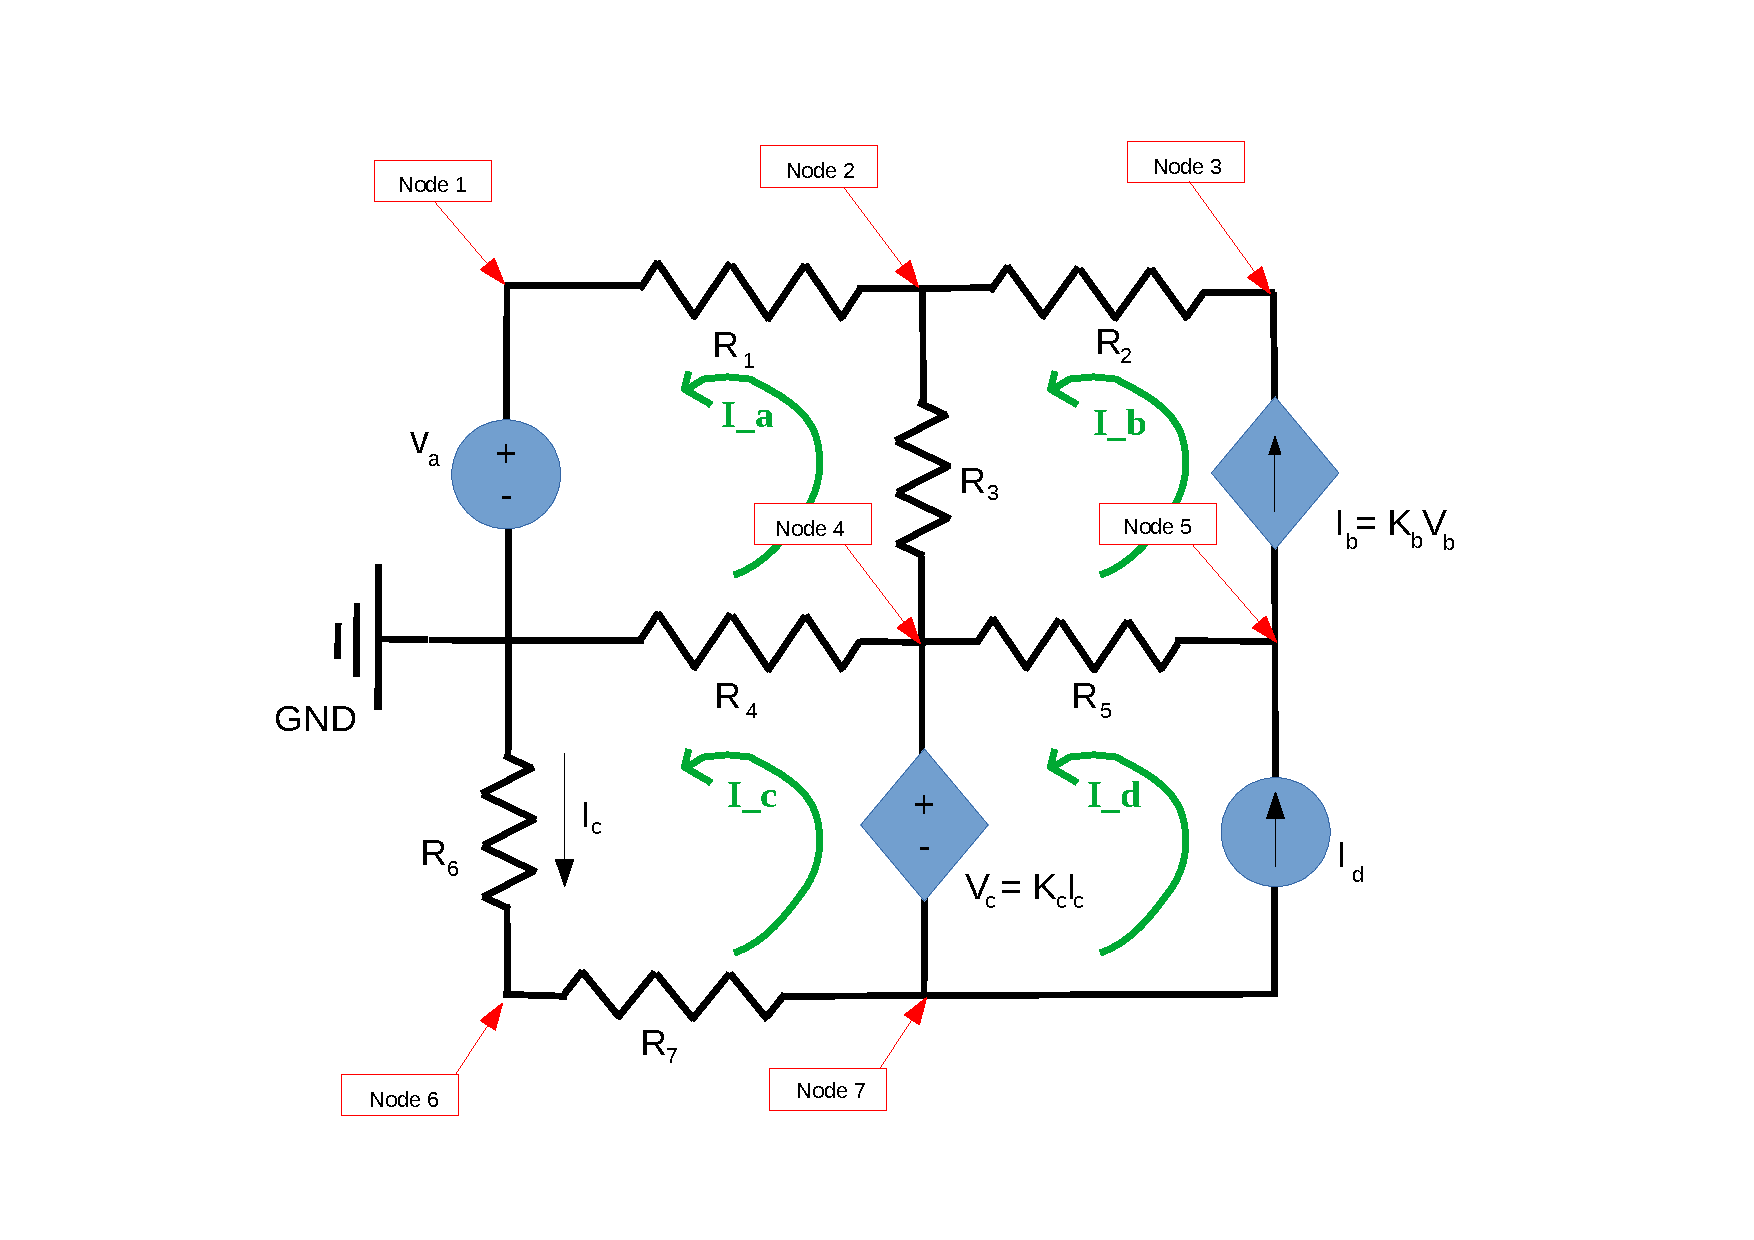
\includegraphics[width=1\linewidth]{rc.pdf}
\caption{Voltage driven serial RC circuit.}
\label{fig:rc}
\end{figure}


\newpage
\section{Theoretical Analysis}
\label{sec:analysis}

In this section, the circuit shown in Figure \ref{fig:rc} is analysed
theoretically, in terms of its response when submited to a voltage in
voltage source $V_a$ and a current in the current source $I_d$, using
Octave.

The circuit consists of four loops, where on the top left loop (loop 1) flows a current $I_a$,
on the top right (loop 2) flows a current $I_b$, on the bottom left (loop 3) a current $I_c$
and on bottom right loop (loop 4) a current $I_d$, all of them assigned to be flowing counterclockwise for
the mesh analysis. The voltage and current sources, $v_a$ and $I_d$, receive countinuous inputs and in order to analyse the circuit
we have to measure the voltage in each node and the current flowing in each loop.
For this purpose we will apply both the Kirchhoff Voltage Law (KVL) and Kirchhoff
Current Law (KCL). \par
Starting the analysis using KVL, we obtain four equations correspondent to each loop:

\begin{equation}
  R_1I_a + R_3(I_a - I_b) + R_4(I_a - I_c) = -v_a ;
  \label{eq:kvl1}
\end{equation}

\begin{equation}
  K_bR_3(-I_a + I_b) - I_b = 0;
  \label{eq:kvl2}
\end{equation}

\begin{equation}
  R_4(-I_a + I_c) + R_6I_c + R_7I_c - K_cI_c = 0;
  \label{eq:kvl3}
\end{equation}

\begin{equation}
  I_d = I_d.
  \label{eq:kvl4}
\end{equation}

Using Octave, we can solve this system of equations easily using matrix operations obtaining the following
solution for the currents:

\begin{table}[h]
  \centering
  \begin{tabular}{|l|r|}
    \hline    
    {\bf Name} & {\bf Value [A or V]} \\ \hline
    Ia & -0.000199\\ \hline 
Ib & -0.000209\\ \hline 
Ic & 0.001001\\ \hline 
Id & 0.001041\\ \hline 
Vb & -0.029341\\ \hline 
Ic & 0.001001\\ \hline 
Ib & -0.000209\\ \hline 
Vc & 8.038843\\ \hline 

  \end{tabular}
  \caption{Results using mesh method}
  \label{tab:tabela1}
\end{table}

As for the analysis using KCL, since we have 8 different nodes we must have 8 different equations
in order to have a solvable system of equations, therefore we obtain the following set of equations:

\begin{equation}
  V_0 = 0;
  \label{eq:kcl1}
\end{equation}

\begin{equation}
  V_1 = V_a;
  \label{eq:kcl2}
\end{equation}

\begin{equation}
  \frac{V_2 - V_1}{R_1} + \frac{V_2 - V_3}{R_2} + \frac{V_2 - V_4}{R_4}= 0;
  \label{eq:kcl3}
\end{equation}

\begin{equation}
  \frac{V_3 - V_2}{R_2} - K_b(V_2 - V_4) = 0;
  \label{eq:kcl4}
\end{equation}

\begin{equation}
  K_b(V_2 - V_4) + \frac{V_5 - V_4}{R_5} = I_d;
  \label{eq:kcl5}
\end{equation}

\begin{equation}
  \frac{V_6}{R_6} + \frac{V_6 - V_7}{R_7} = 0;
  \label{eq:kcl6}
\end{equation}

\begin{equation}
  V_4 - K_c\frac{V_6}{R_6} - V_7 =0;
  \label{eq:kcl7}
\end{equation}

\begin{equation}
  \frac{V_4}{R_4} + \frac{V_4 - V_2}{R_3} + \frac{V_4 - V_5}{R_5} + \frac{V_7 - V_6}{R_7} = -I_d,
  \label{eq:kcl8}
\end{equation}

being \textbf{Equation \ref{eq:kcl1}} referent to node 0,\textbf{Equation \ref{eq:kcl2}} to node 1, \textbf{Equation \ref{eq:kcl3}} to node 2,
\textbf{Equation \ref{eq:kcl4}} to node 3, \textbf{Equation \ref{eq:kcl5}} to node 5, \textbf{Equation \ref{eq:kcl6}} to node 6, \textbf{Equation \ref{eq:kcl7}}
to the linear current dependent voltage source and \textbf{Equation \ref{eq:kcl8}} to the sum of both nodes 4 and 7.

Using Octave, we can solve this system of equations easily using matrix operations obtaining the following
solution for the voltages:

\begin{table}[h]
  \centering
  \begin{tabular}{|l|r|}
    \hline    
    {\bf Name} & {\bf Value [A or V]} \\ \hline
    V0 & 0.000000\\ \hline
V1 & 5.195199\\ \hline
V2 & 4.989875\\ \hline
 V3 & 4.556619\\ \hline
V4 & 5.019215\\ \hline
V5 & 8.853743\\ \hline
V6 & -2.012617\\ \hline
V7 & -3.019628\\ \hline
Ic & 0.001001\\ \hline
Ib & -0.000209\\ \hline

  \end{tabular}
  \caption{Results using nodes method}
  \label{tab:tabela2}
\end{table}

As expected from theory, both methods present the same results as can be seen in tables \ref{tab:tabela1} and \ref{tab:tabela2}.


\newpage
\section{Simulation Analysis}
\label{sec:simulation}


\begin{table}[h]
  \centering
  \begin{tabular}{|l|r|}
    \hline    
    {\bf Name} & {\bf Value [A or V]} \\ \hline
    @gb[i] & -2.08664e-04\\ \hline
@id[current] & 1.041397e-03\\ \hline
@r1[i] & 1.992363e-04\\ \hline
@r2[i] & 2.086637e-04\\ \hline
@r3[i] & -9.42740e-06\\ \hline
@r4[i] & 1.200363e-03\\ \hline
@r5[i] & -1.25006e-03\\ \hline
@r6[i] & 1.001127e-03\\ \hline
@r7[i] & 1.001127e-03\\ \hline
v(1) & 5.195199e+00\\ \hline
v(2) & 4.989875e+00\\ \hline
v(3) & 4.556619e+00\\ \hline
v(4) & 5.019215e+00\\ \hline
v(5) & 8.853743e+00\\ \hline
v(6) & -2.01262e+00\\ \hline
v(7) & -3.01963e+00\\ \hline
v(8) & -2.01262e+00\\ \hline

  \end{tabular}
  \caption{Operating point. A variable preceded by @ is of type {\em current}
    and expressed in Ampere; other variables are of type {\it voltage} and expressed in
    Volt.}
  \label{tab:tabela3}
\end{table}



Table~\ref{tab:tabela3} shows the simulated operating point results for the circuit
under analysis. Compared to the theoretical analysis results, the simulation analysis results are the same
due to all components having a linear behaviour.






\section{Conclusion}
\label{sec:conclusion}

In this laboratory assignment the objective of analysing the mentioned circuit has been
achieved. Voltages and Current static analyses have been performed both
theoretically using the Octave tools and by circuit simulation using the
Ngspice tools. The simulation results matched the theoretical results
precisely and both theoretical analyses produce consistent results. The reason for this perfect match is the fact that this is a
straightforward circuit containing only linear components, so the theoretical
and simulation models cannot differ.



%\cleardoublepage

% ----------------------------------------------------------------------
%  Bibliography
% ----------------------------------------------------------------------
%\addcontentsline{toc}{section}{\bibname}
%\bibliographystyle{abbrvunsrtnat} % <<<<< SELECT IF USING REFERENCES BY NUMBER (CITATION ORDER)
%\bibliography{../../../BIBfile.bib}

% ----------------------------------------------------------------------
\end{document}
% ----------------------------------------------------------------------
